\documentclass[10pt,a4paper,twoside]{article}
\usepackage[dutch]{babel}
%laad de pakketten nodig om wiskunde weer te geven :
\usepackage{amsmath,amssymb,amsfonts,textcomp,amsthm}
%laad de pakketten voor figuren :
\usepackage{graphicx}
\usepackage{multirow}
\usepackage{float,flafter}
\usepackage{lmodern}
\usepackage{hyperref}
\usepackage{inputenc}
\usepackage{subcaption}
\usepackage{biblatex} %Imports biblatex package\
\usepackage{csquotes}
\addbibresource{sources.bib}
\usepackage[T1]{fontenc}
\usepackage{lmodern}
%zet de bladspiegel :
\setlength\paperwidth{20.999cm}\setlength\paperheight{29.699cm}\setlength\voffset{-1in}\setlength\hoffset{-1in}\setlength\topmargin{1.499cm}\setlength\headheight{12pt}\setlength\headsep{0cm}\setlength\footskip{1.131cm}\setlength\textheight{25cm}\setlength\oddsidemargin{2.499cm}\setlength\textwidth{15.999cm}

\begin{document}
\begin{center}
\hrule

\vspace{.4cm}
{\bf {\Huge AD2 Verslag}}
\vspace{.2cm}
\end{center}
\begin{center}
{\bf{\Large invloed heaps op kortste pad algoritme}}
\end{center}
{\bf Ben De Meurichy}  \\
\hspace{\fill} 4/12/2023 \\
\hrule
%\bf genereert vette letters, \large \Large \huge \Huge \tiny \small ... verschillende lettergroottes, met \em, \it, \sl krijg je cursieve tekst
%Je moet accolades gebruiken om aan te geven waarop je het commando precies wil laten inwerken.
% commentaar zet je in de tex-file met een %-tekentje voor.


\section{ Theorievragen}
Het tweede algoritme om de decreasekey bewerking uit te voeren zal een betere tijdcomplexiteit hebben omdat we hier enkel de twee kinderen van $S_v$ met elkaar moeten mergen als deze er beiden zijn en 1 top moeten toevoegen tot S.\\
In tegenstelling tot algoritme 1 waarbij we de hele subboom $S_v$ verwijderen, dan S te herstellen en dan heel $S_v$ te mergen met S. Dit zal over het algemeen meer werk kosten dan de twee kleinere merge bewerkingen in algoritme twee.
Algoritme twee garandeerd niet altijd dat de heap die hier uit komt een skew heap is, als we een blad verwijderen uit de heap dat een linkerkind van zijn ouder is, hebben we geen heap meer om op deze plaats terug te plaatsen en voldoet de achtergebleven heap niet meer aan de skew eigenschap. We zullen zien in de volgende bewijzen dat het moeilijker is om bij algoritme twee een slechte top (een top met meer toppen in het rechterkind dan in het linkerkind) te creëren dan bij algoritme 1 wat er voor zorgt dat de heap bij algoritme twee over het algemeen beter gebalanceerd is.

\subsection{Algoritme 1}
\begin{proof}
Als we de beschrijving van het algoritme opsplitsen in de volgende drie stappen kunnen we het bewijs stelling 16 gebruiken in de cursus om de geamortiseerde tijdcomplexiteit te berekenen van een reeks van n bewerkingen op een initieel lege skew heap:
\begin{itemize}
    \item verwijder de subboom $S_v$ met wortel v uit de skew heap S
    \item herstel de skew eigenschap op het pad van v naar de wortel van S
    \item merge $S_v$ met herstelde S
\end{itemize}
De kost die nog niet bewezen is hierbij, is de kost van het herstellen van S en het verwijderen van $S_v$.\\
Het verwijderen van de subboom zal zorgen voor slechte toppen in S als v op het linkerpad van de top lag en voor goede toppen als deze op het rechterpad van de top lag.\\
Dit wordt opgelost door het herstellen van de achtergebleven heap. Om deze reden berekenen we de kost van deze bewerkingen samen. Aangezien de echte kost van deze bewerking enkel het overlopen van het pad van v naar de wortel is voor het herstellen (de pointers verwijderen naar v uit de heap is verwaarloosbaar als kost), maar de potentiaal wel drastisch kan veranderen door $S_v$ te verwijderen is het makkelijker om deze samen te beschouwen zodat we beperkingen kunnen opleggen op de gewijzigde kost.\\
De herstelbewerking wordt als volgt beschreven: "Als een top op het pad van v naar de wortel v in zijn linkerdeelboom heeft en een rechterkind heeft, dan worden de kinderen gewisseld".\\
Dit kunnen we gebruiken in de redenering bij het verwijderen van $S_v$.\\
Door de verwijder bewerking kunnen sommige toppen waarvan v in het rechterkind zat goed worden en toppen met v in het linkerkind slecht worden. Na het herstellen worden de toppen die slecht werden terug goed dus dan hebben we als potentiaal $\Phi(D')-\Phi(D)\leq0$. Als de tabel uit het bewijs van stelling 16 wordt uitgebreid met deze bevinding kunnen we dan de geamortiseerde kost van de decreasekey bewerking bewijzen door de kost van alle stappen op te tellen. De herstelbewerking moet in het slechtste geval $n-1$ toppen overlopen, dit is het geval wanneer de initiele heap S een heap is met alle toppen op het linkerpad.

\begin{table}[H]
\begin{tabular}{lllll}
\cline{1-3}
\multicolumn{1}{|l|}{}                                                                                         & \multicolumn{1}{l|}{echte kost}                        & \multicolumn{1}{l|}{gewijzigde kost}                                    &  &  \\ \cline{1-3}
\multicolumn{1}{|l|}{\begin{tabular}[c]{@{}l@{}}deelboom Sv uit S verwijderen \\ en S herstellen\end{tabular}} & \multicolumn{1}{l|}{\# toppen van v tot de wortel = T} & \multicolumn{1}{l|}{$(T)+\Phi(D')-\Phi(D)\leq(T)$} &  &  \\ \cline{1-3}
                                                                                                               &                                                        &                                                                         &  &  \\
                                                                                                               &                                                        &                                                                         &  & 
\end{tabular}
\end{table}
Dit betekent dus dat de geamortiseerde kost voor de decreasekey bewerking gelijk is aan die van de merge bewerking plus de kost van het verwijderen en herstellen van de boom die we net hebben bewezen. Als we dan de conclusie van het bewijs van stelling 16 gebruiken zien we dat de decreasekey bewerking de hoogste kost heeft met geamortiseerd $n*(n+\log(n))$ kost, dus $O(n^2)$. Dit geeft ons dus een kost terug van $O(n)$ per bewerking.
\end{proof}
\subsection{Algoritme 2}
\begin{proof}
We kunnen dit idee om de geamortiseerde kost analyse uit te voeren ook gebruiken om de complexiteit te bewijzen met algoritme 2.\\
Hier splitsen we de bewerking in de stukken:
\begin{itemize}
    \item verwijder top v uit S
    \item merge kinderen van v tot 1 subboom $S_v'$
    \item plaats $S_v'$ op de plaats van v in heap S
    \item merge S en top v met verlaagde prioriteit
\end{itemize}
De 2 merge stappen hoeven we niet meer te bewijzen omdat deze overeen komen met de reeds bewezen delen uit het bewijs van stelling 16 in de cursus. Het plaatsen van $S_v'$ heeft als echte kost 1 maar de gewijzigde kost kan hier wel veranderen. Het mergen van de 2 kinderen van v zorgt dat de boom $S_v'$ minder slechte toppen heeft dan $S_v$ (deelresultaat 4).\\
Hieruit volgt dat $\Phi(D')-\Phi(D)\leq0$ (\textbf{deelresultaat 5}) als we de invloed van het verwijderen van v uit S appart zien .\\
Hierbij kunnen er wel slechte toppen bijkomen. Dit is het geval als v in het linkerkind van een top zit en er in het rechterkind exact evenveel toppen zaten. Het slechtste geval hiervoor kan dus een bovengrens vormen voor de hoeveelheid goede toppen die hiermee slecht gemaakt kunnen worden. Dit is wanneer de heap de vorm heeft van een perfect gebalanceerde binaire boom en we de top verwijderen die het meest linkerkind is van de wortel (ook al is het resultaat van het "terugplaatsen van de kinderen" hier geen skew heap).
\\
Het aantal goede toppen dat hiermee slecht wordt gemaakt zijn alle toppen van v tot de wortel, dit is dus gelijk aan de diepte van v wat gelijk is aan $\log(n)$ (\textbf{deelresultaat 6}). Met deze bevindingen kunnen we de tabel uit het bewijs van stelling 16 uitbreiden om alle stappen van de decrease key bewerking te sommeren om zo tot een bovengrens voor de kost te bekomen.
\begin{table}[H]
\begin{tabular}{lllll}
\cline{1-3}
\multicolumn{1}{|l|}{}                                   & \multicolumn{1}{l|}{echte kost} & \multicolumn{1}{l|}{gewijzigde kost}                  &  &  \\ \cline{1-3}
\multicolumn{1}{|l|}{deelboom $S_v'$ terugplaatsen in S} & \multicolumn{1}{l|}{1}          & \multicolumn{1}{l|}{$1+\Phi(D')-\Phi(D)\leq1$ (deelresultaat 5)}        &  &  \\ \cline{1-3}
\multicolumn{1}{|l|}{verwijder v uit S}                  & \multicolumn{1}{l|}{1}          & \multicolumn{1}{l|}{$1+\Phi(D')-\Phi(D)\leq\log(n) $(deelresultaat 6)} &  &  \\ \cline{1-3}
                                                         &                                 &                                                       &  & 
\end{tabular}
\end{table}
Nu kan de kost berekent worden door de kost van alle stappen op te tellen. Hierbij kunnen we de conclusie van het bewijs van stelling 16 terug gebruiken en bekomen we voor een reeks van n bewerkingen op een initieel lege skew heap $n*(\log(n)+\log(n)+\log(n))$ met 2 keer $\log(n)$ van de merge bewerkingen en 1 keer van het verwijderen van top v uit S.\\
Dit geeft een geamortiseerde bovengrens van $O(n\log(n)$ voor n bewerkingen dus $O(\log(n))$ per bewerking.
\end{proof}
\newpage
\section{Heaps implementatie}
\subsection{Skew heap}
Om te voldoen aan de opgave voor de skew heap is er een vrij standaard skew heap geïmplementeerd.
De details die open zijn voor interpretatie zoals de merge- en decreasekey-bewerkingen zal ik wel toelichten.
\\\\
Voor het mergen van twee skew heaps is gekozen om de recursieve top-down methode te gebruiken uit de cursus.
De complexiteit hiervan is geamortiseerd $O(\log{}n)$ (bewijs stelling 16 cursus). \\Door het eenvoudige idee heeft dit geen moeilijkheden gegeven bij de implementatie.
\\\\
Bij de {\fontfamily{lmss}\selectfont decreaseKey} operatie is gekozen voor het eerste voorstel in de theorievragen uit de opgave.
Door de deelboom met het element waarop {\fontfamily{lmss}\selectfont decreaseKey} wordt opgeroepen als wortel te nemen en deze volledig te verwijderen uit de totale boom, moeten we de overgebleven heap terug een skew heap maken.\\
Doordat alle subbomen van een skew heap ook skew heaps zijn hoeven we enkel te kijken naar de ouder van de wortel die we net hebben verwijderd, wat vanzelfsprekend volgt uit de skew heap eigenschap (als een top een rechterkind heeft, heeft deze ook een linkerkind).\\ 
De skew eigenschap zal enkel geschonden worden als de subboom een linkerkind was van de ouder.\\
Er moet dus enkel gecontroleerd worden of dit het geval is om twee volledige skew heaps te bekomen die gemerged kunnen worden.\\
De achtergebleven skew heap zal waarschijnlijk geen skew heap zijn die bekomen kan worden door normale toevoegbewerkingen maar voldoet wel aan de regels die worden opgelegd door de skew eigenschap. Het mergen van de twee subbomen hebben we eerder al besproken.
\\\\
Ik heb gekeken of er een groot verschil is in snelheid tussen enkel de ouder terug skew te maken of het pad tot de wortel af te gaan en zolang de verwijderde top in de linkerboom van deze top zit en er een rechterkind is de kinderen te wisselen zoals in de opgave staat.\\
Dit zou theoretisch gezien tot een betere skew heap moeten leiden die meer naar links is gebalanceerd. Ik heb dit opgenomen in de optimalisaties.
\\\\
\begin{figure}[h]
\begin{subfigure}{0.34\textwidth}
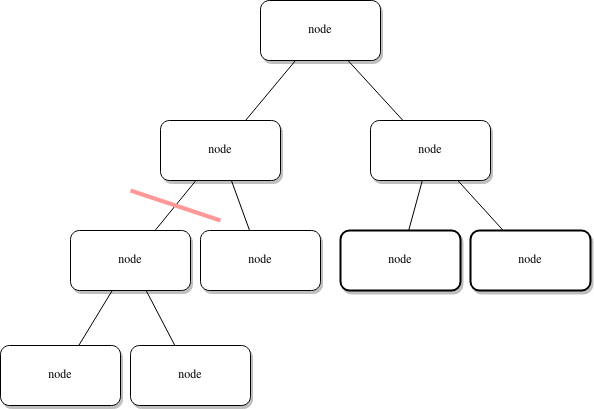
\includegraphics[width=0.9\linewidth]{figures/skewheap.drawio.png}
\caption{begin heap}
\label{fig:beginHeap}
\end{subfigure}
\begin{subfigure}{0.34\textwidth}
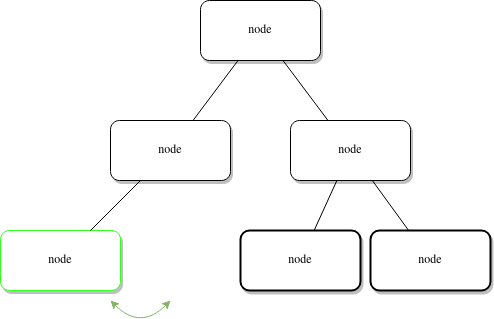
\includegraphics[width=0.9\linewidth]{figures/skewheapNoOpt.drawio.png}
\caption{bekijk enkel ouder}
\label{fig:noOpt}
\end{subfigure}
\begin{subfigure}{0.34\textwidth}
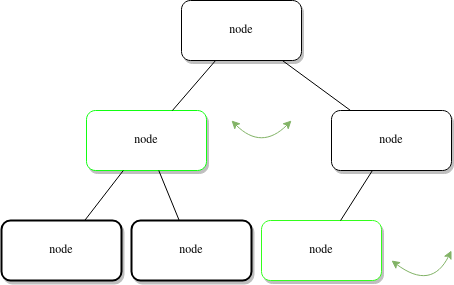
\includegraphics[width=0.9\linewidth]{figures/skewheapOpt.drawio.png}
\caption{volledige optimalisatie}
\label{fig:Opt}
\end{subfigure}
\caption{Overgebleven heap na verwijderen subboom}
\end{figure}

\subsection{Leftist heap}
Als tweede heap heb ik gekozen voor de leftist heap.\\
Aangezien dit eigenlijk een skew heap is met een strengere skew eigenschap, wilde ik zien of deze theoretisch beter gebalanceerde heap ook beter presteert in de praktijk.
\\\\
Als merge bewerking heb ik gekozen om ook hiervoor een recursieve oplossing te zoeken.\\
Dit leek gemakkelijker in programmeerwerk en hierdoor was het niet nodig om tussentijdse structuren op te slaan.\\
Het nadeel aan deze aanpak is wel dat er recursief wordt gewerkt, dit brengt op zich overhead met zich mee door steeds nieuwe functie-oproepen te doen. Omdat we hiermee de nullpadlengtes kunnen aanpassen terwijl we de heaps aan het mergen zijn leek het me toch de moeite om dit zo te implementeren in plaats van zoals in de cursus. Het idee komt grotendeels overeen met dat van de skew heap. Het grote verschil is de extra controle van de nullpadlengte met het eventuele wisselen van de kinderen van de top.
\\\\
Door de {\fontfamily{lmss}\selectfont decreaseKey} functie op een gelijkaardige manier te implementeren zoals bij de skew heap komt er een probleem bij. De achtergebleven heap moet terug een leftist heap worden. Dit is iets complexer dan bij de skew heap maar de nullpadlengten kunnen vrij efficient terug in orde gebracht worden\cite{decreaseKeyLeftist}.
\\\\
Om van de achtergebleven heap terug een leftist heap te maken moeten de kinderen moeten gewisseld worden als er geen linkerkind is of als de top beide kinderen heeft en de nullpadlengte van het rechterkind groter is dan die van het linkerkind. Door daarna de nullpadlengte van de top in te stellen op het minimum van beide kinderen plus een (als een kind mist is de nullpadlengte gelijk aan nul). Dit moeten we blijven herhalen op het volledige pad tot de wortel.\\
Gelukkig kan hier ook vroeger gestopt worden. Als we ons in een top bevinden die het linkerkind $l$ is van de oudere en de ouder heeft ook een rechterkind $r$ waarvoor geldt $npl(l)\geq npl(r)$, dan betekent dit dat de ouder de nullpadlengte + 1 van $r$ moet bevatten want $npl(top)=min(npl(l),npl(r))+1$.\\
Door deze eigenschap kunnen we het herstellen van de leftist heap vroegtijdig beëindigen en besparen we tijd. Dit is een optimalisatie waar ik op voorhand heb achter gezocht dus hier heb ik geen implementatie zonder optimalisatie van.
\\\\
Het mergen van de twee leftist heaps die voortkomen uit de {\fontfamily{lmss}\selectfont decreaseKey} wordt gedaan zoals hierboven wordt beschreven.
\\\\
\begin{figure}[H]
    \begin{subfigure}{0.5\textwidth}
        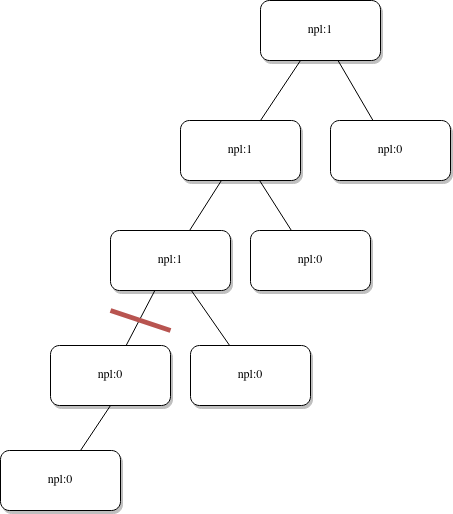
\includegraphics[width=0.9\linewidth]{figures/leftistBefore.drawio.png}
        \caption{Leftist heap voor {\fontfamily{lmss}\selectfont decreaseKey}}
        \label{fig:LeftistHeapBefore}
    \end{subfigure}
    \begin{subfigure}{0.5\linewidth}
        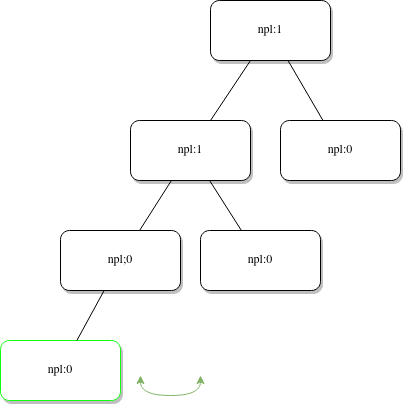
\includegraphics[width=0.9\linewidth]{figures/leftistHeapRepaired.drawio.png}
        \caption{Repaired leftist heap}
        \label{fig:LeftistHeapRepaired}
    \end{subfigure}
    \caption{Herstelbewerking op leftist heap (deel van {\fontfamily{lmss}\selectfont decreaseKey})}
\end{figure}

\section{Kortste pad implementatie}
Het kortste pad algoritme is een eenvoudige implementatie van Dijkstra 's kortste pad algoritme.\\
De interne representatie wordt weergegeven door een hashmap van de buren voor elke top. Deze wordt verwerkt door eerst alle toppen in de map te steken en dan alle bogen.\\
Het verwerken van de graaf neemt dus $\Theta(|E|+|V|)$ (met E en V respectievelijk de verzameling bogen en toppen in de graaf) tijd in beslag zoals vermeld werd in de opgave.
\\\\
Het algoritme zelf is zonder eigenaardigheden geprogrammeerd.\\
Wat wel afwijkt van een standaard implementatie is de map die bijhoudt welk element uit de wachtlijn overeen komt met welke top omdat de {\fontfamily{lmss}\selectfont decreaseKey} opgeroepen wordt op de elementen in de wachtrij dus hier moeten we dan ook aan geraken wanneer we de top hebben gegeven.
\\\\
Door {\fontfamily{lmss}\selectfont decreaseKey} vaak te gebruiken verwacht ik een minimaal verschil omdat deze op beide heaps een tijdcomplexiteit van $O log(n)$ heeft. De theoretische tijdcomplexiteit is bij beide heaps dezelfde maar ik wilde zien of de constanten in de praktijk misschien veel verschillen.
\section{Bespreking metingen}
Om de uitvoeringstijd te meten van de operaties heb ik voor elke belangrijke operatie op de heap reeksen van 0 tot 10 000 000 bewerkingen laten uitvoeren. Dit geeft dus de geamortiseerde kost terug van deze bewerking.
\\\\
Bij de toevoegbewerking \ref{fig:addBench} zien we een vrij groot verschil tussen de skew en leftist heap. Uit de test kunnen we afleiden dat ze beiden geamortiseerd $O n\log(n)$ dus per toevoegbewerking $O \log(n)$.\\
De leftist heap zal wel betere constanten hebben waardoor deze zo veel sneller is. Het kan ook zijn dat een aantal elementen op volgorde toevoegen beter uitkomt voor de leftist heap maar dit blijkt niet uit het achterliggende idee.\\
Het verschil tussen de skew heap met en zonder optimalisatie is minimaal. Dit ligt vanzelfsprekend aan dat de optimalisatie bij {\fontfamily{lmss}\selectfont decreaseKey} zit en die hier niet wordt gebruikt.\\
Als we bij deze benchmark het aantal vergelijkingen bekijken \ref{fig:addBenchComp} zien we wel dat de Leftist heap wel redelijk wat meer vergelijkingen doet. Dit is logisch omdat deze natuurlijk moet garanderen dat de heap leftist blijft.
\\\\
Het verwijderen van het kleinste element uit de heap heeft weinig tot geen verschil tussen de verschillende heaps. Dit komt doordat bij alle heaps beide subbomen van de wortel volledig gemerged moeten worden. Aangezien deze bewerking bij beide heaps gelijkaardig zijn geimplementeerd is het te verwachten dat deze ongeveer even goed presteren als ze gelijkaardige heaps moeten mergen.\\
Door de optimalisatie is het ook te verwachten dat de skew heap meer op een leftist heap zal lijken of zelfs vaak een leftist heap zal zijn. Ook hier is het vergelijkingen bij de leftist heap meer dan bij de skew heap door dezelfde reden, dit zal ook zo zijn in de volgende benchmarks \ref{fig:decreaseKeyBenchComp}.
\\\\
De {\fontfamily{lmss}\selectfont decreaseKey} operatie \ref{fig:decreaseKeyBench} heeft de meest verrassende resultaten. Hierbij presteert de leftist heap beter dan beide versies van de skew heap. Dit zal waarschijnlijk deels aan de benchmark liggen die geen gerandomiseerde data gebruikt en deels ook aan implementatiedetails die voor extra overhead zorgt bij de skew heaps.\\
De leftist heap zal beter gebalanceerd zijn waardoor het mergen van de subbomen op deze heap minder tijd in beslag neemt. Het verschil tussen de geoptimaliseerde skew heap en de niet geoptimaliseerde is weer minimaal, we kunnen dus niet met zekerheid zeggen of dit wel iets opbrengt.\\
Dit komt doordat de optimalisatie niet zo ingrijpend is.
Als we nu beide heaps in een kortste pad algoritme \ref{fig:shortestPathGraph} gebruiken merken we op dat geen van beide heaps beter presteert dan de andere. De grafieken lijken exponentieel doordat de gebruikte grafen een rooster zijn zijn van $nxn$ toppen die allemaal verbonden zijn met hun buren via de bogen
$$buren(N_{ij})=\begin{cases}
       \text{graaf[i-1][j]}\\
       \text{graaf[i][j-1]}
     \end{cases} met i,j=0,1,...,n$$
De eigenlijke complexiteit zal dus dichter bij $O(n\log(n))$ liggen wat de theoretische tijdcomplexiteit is van het kortste pad algoritme van Dijkstra ($O((E+V)\log(V))$ met E de bogen en V de toppen in de graaf).
Door de opstelling van de graaf zijn de operaties die op de heaps worden opgeroepen bijna hetzelfde en krijgen we gelijkaardige resultaten.\\
De prestaties van het algoritme hangen ook meer af van de implementatie van het algoritme zelf in plaats van die van de heaps. Als er een graaf is waarvoor de {\fontfamily{lmss}\selectfont decreaseKey} functie vaak aangeroepen zou worden zouden we misschien een kleine verbetering in uitvoertijd kunnen zien bij de leftist heap.


\section{Besluit}
Hoewel er duidelijk verschil zit op de prestaties van beide heaps heeft dit maar een minimale invloed op het uitvoeren van het kortste pad algoritme van Dijkstra. Dit kan verklaard worden door de tijdcomplexiteit van Dijkstra's algoritme.\\
De heap waarbij ik misschien wel nog een verschil zou verwachten zou de fibonacci heap zijn. Deze heeft theoretisch gezien voor alle bewerkingen buiten het kleinste element verwijderen een tijdcomplexiteit van $O(1)$. Beide heaps die ik heb vergeleken hadden voor toevoeg,verwijder en decreaseKey bewerking een theoretische tijdcomplexiteit van $O(log(n))$.
\newpage

\section{Appendix-grafieken}

\subsection{tijd}

\begin{figure}[H]
    \centering
    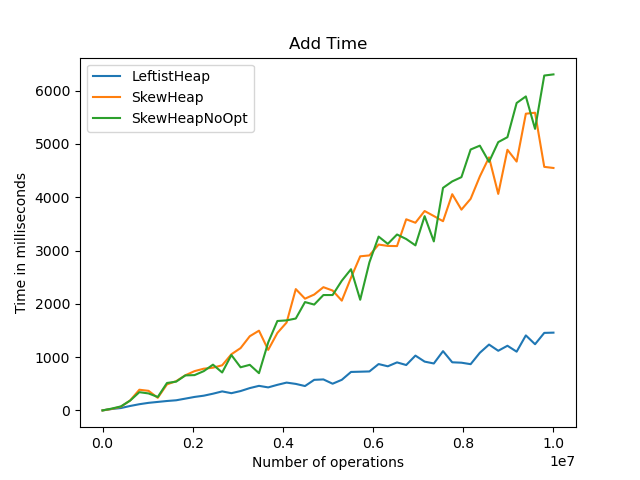
\includegraphics[width=0.85\linewidth]{graphs/AddTime.png}
    \caption{uitvoertijd van reeksen toevoegbewerkingen}
    \label{fig:addBench}
\end{figure}
\begin{figure}[H]
    \centering
    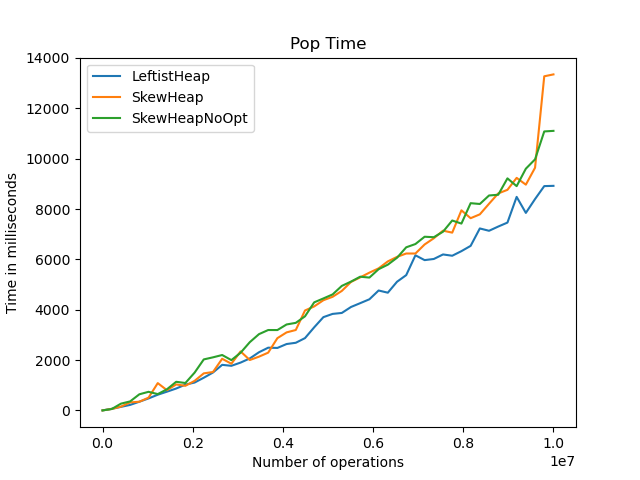
\includegraphics[width=0.85\linewidth]{graphs/PopTime.png}
    \caption{uitvoertijd van reeksen popBewerkingen}
    \label{fig:popBench}
\end{figure}
\begin{figure}
    \centering
    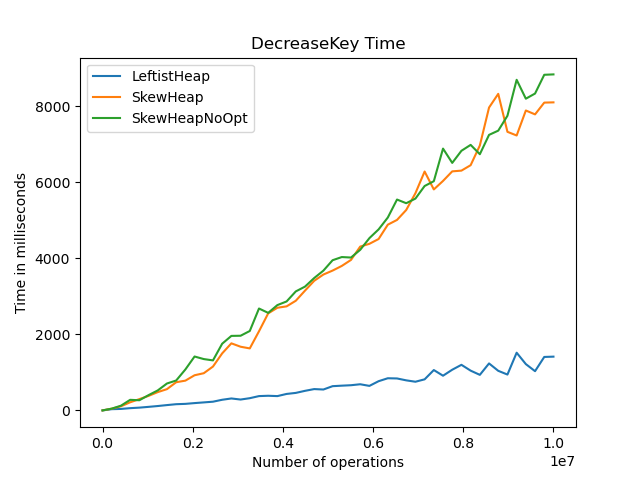
\includegraphics[width=0.85\linewidth]{graphs/DecreaseKeyTime.png}
    \caption{uitvoertijd van reeksen decreaseKeyBewerkingen}
    \label{fig:decreaseKeyBench}
\end{figure}

\subsection{vergelijkingen}
\begin{figure}[H]
    \centering
    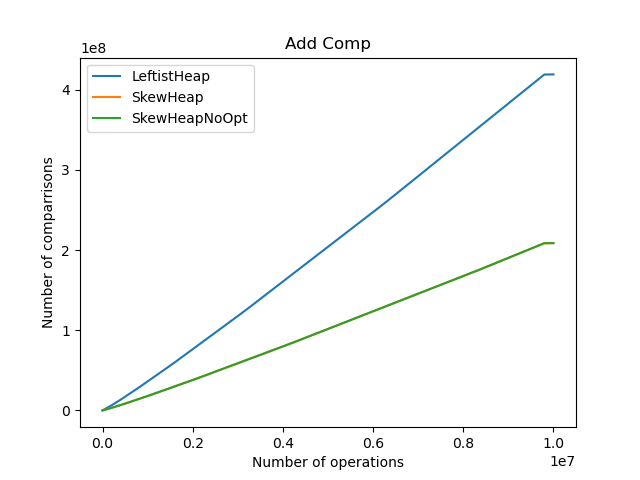
\includegraphics[width=0.85\linewidth]{graphs/AddComp.png}
    \caption{aantal vergelijkingen bij reeksen toevoegbewerkingen}
    \label{fig:addBenchComp}
\end{figure}
\begin{figure}
    \centering
    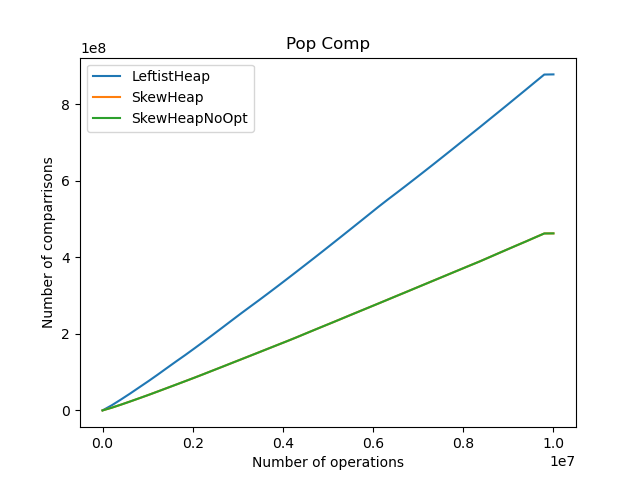
\includegraphics[width=0.85\linewidth]{graphs/PopComp.png}
    \caption{aantal vergelijkingen bij reeksen popBewerkingen}
    \label{fig:popBenchComp}
\end{figure}
\begin{figure}
    \centering
    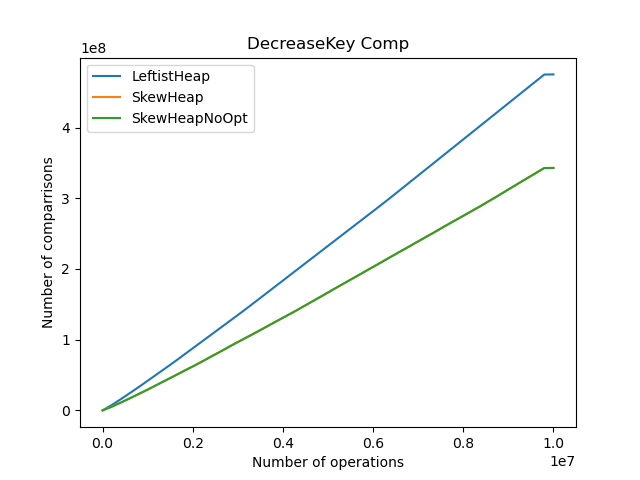
\includegraphics[width=0.85\linewidth]{graphs/DecreaseKeyComp.png}
    \caption{aantal vergelijkingen bij reeksen decreaseKeyBewerkingen}
    \label{fig:decreaseKeyBenchComp}
\end{figure}

\subsection{kortste pad}
\begin{figure}[H]
    \centering
    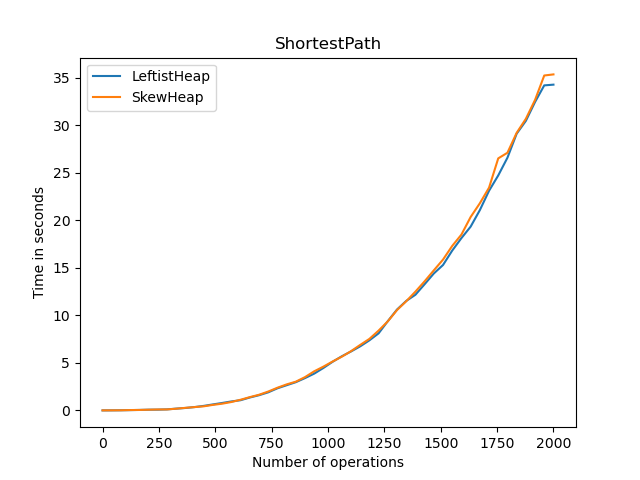
\includegraphics[width=0.85\linewidth]{graphs/ShortestPath.png}
    \caption{Kortste pad benchmark van 1x1 tot 2000x2000 raster}
    \label{fig:shortestPathGraph}
\end{figure} 

\section{Bronnen}
\printbibliography
\end{document}